\pagebreak
\subsection{Electrical Design}

\subsubsection{Block Diagram}
\label{sec:4.5.1}

The electronics design can be seen in Figure \ref{fig:electronics-block-diagram} which shows the connections, grounding, voltages, and signals. 

\begin{figure}[H]
    \begin{align*}
        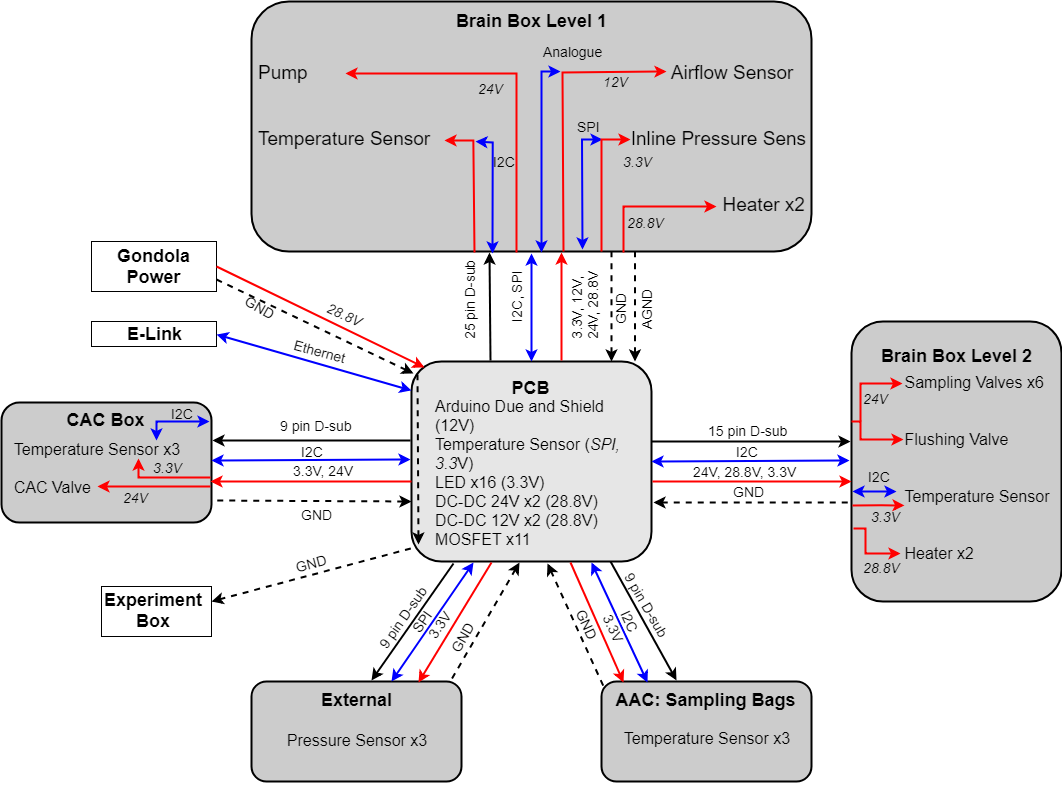
\includegraphics[width=16cm]{block-diagram-2.png}
    \end{align*}
    \caption{Block Diagram for all Electronic Components Showing the Connection, Signal and Power Connections.}\label{fig:electronics-block-diagram}
\end{figure}

Most of the electronics will be located in the Brain inside the AAC box. However, there will be six distinct areas:

\begin{enumerate}
    \item The Brain level 3, where the PCB is located with the Arudino and shield, two 24 V DC-DC, one 12 V voltage regulator, one temperature sensor, 11 MOSFETs and 14 LEDs.
    \item The Brain level 2, where the valve manifolds with six sampling valves\footnote{There will be eight valves connected mechanically in the manifold to ensure it is sealed but only six will be connected to the bags and electronics.\label{fn:extravalve}}, the flushing valve, one heater and one temperature sensor are located.
    \item The Brain level 1, where the pump, airflow sensor and sensor box containing 3 pressure sensors, 1 temperature sensor and 1 humidity sensor are located.
    \item The AAC box, where 3 ambient temperature sensors are located.
    \item The CAC box, where the CAC valve and 3 ambient temperature sensors are located.
    \item Outside of the experiment box, where 3 ambient pressure sensors are located.
\end{enumerate}

From the PCB, on level 3, five D-sub connectors will be used to connect to the other five areas. A 25 pin connector will be used for level 1, 15 pin connector will be used for level 2 and nine pin connectors will be used for the CAC box, AAC box sampling bags area, and the external pressure sensors. In addition there will be a connection to the gondola power and gondola E-link.

All of the power distribution will take place on the PCB using two 24 V DC-DC converters in parallel with a forwarding diode which feed a 12 V voltage regulator. 
\begin{itemize}
  \item $28.8 \, V \Longrightarrow 24 \, V $ By DC-DC converters
  \item $24 \, V \Longrightarrow 12 \, V$ By voltage regulator
  \end{itemize}
The heaters will not require the voltage to be stepped down and so will be powered directly from the gondola battery.

The Arduino will control all of the sensors, valves, heaters and the pump from the PCB. Sensors will be directly connected to the Arduino. The valves, heaters and the pump will be connected via a switching circuit.

The LEDs are used as visual indicators that display whether different parts of the circuit are alive or not. They give indications on the status of the valves, pump, heaters, DC-DC converters and Arduino. 

Grounding will be following a distributed single point grounding, with all ground connections meeting at a single star point to ensure there are no floating grounds. As not all components are connected via DC-DC converters the experiment will not be isolated from the gondola power supply therefore there will be a connection between the star point and the gondola ground. The star point will be located on the main PCB board which will then be grounded to the experiment box. The grounding can be seen in Figure \ref{fig:electronics-block-diagram} where it is indicated by dashed lines labeled GND. 

\subsubsection{Miniature Diaphragm Air Pump}
The pump which has been selected is the 850.1.2. KNDC B, Figure \ref{fig:pumppic}, which is manufactured by KNF. One of the reasons this pump has been selected is that it has successfully been flown on a similar flight in the past where it managed to pump enough air at 25 km altitude to have 180 mL remaining at sea level \cite{LISA}. However, to ensure the pump will operate as intended, several tests will still be carried out. These tests --- 4, 5, 18, 28 and 29, can be seen in Tables \ref{tab:vacuum-test}, \ref{tab:thermal-test}, \ref{tab:pump-low-pressure-test}, \ref{tab:pump-operation-test}, and \ref{tab:pump-current-pressure-test}. The pump has already passed three of these tests and their results can be seen in Section \ref{sec:test28result} for Test 28, Section \ref{subsection:pumplowpressuretest} for Test 18 and Section \ref{sec:test29result} for Test 29.

At sea level conditions the pump was tested and found to have a flow rate of 8.0 L/min and a current draw of 250 mA. The peak current draw was recorded as 600 mA which lasts for less than one second and occurs when the pump is switched on. 

From the results of Test 18, in Section \ref{subsection:pumplowpressuretest}, the flow rate is estimated to be 3.0 L/min at the lowest pressure that will be seen in flight. This is in line with requirement D23. The results found in Test 28, in Section \ref{sec:test28result}, appear to be inline with the information given by the manufacturer, seen in Figure \ref{fig:pumpflowcur}.  The highest continuous current draw expected from the pump is 185 mA when the experiment is at 12 km altitude and is expected to decrease as we increase in altitude. While it appears the pump increases in current draw at around 6 km there is no plan to sample below 12 km therefore the highest current draw can be taken from 12 km. As the pump has a peak current of 600 mA when it switches on, the mosfet and DC-DC power have been chosen to be able to withstand this demand. 

\begin{figure}[H]
    \begin{align*}
        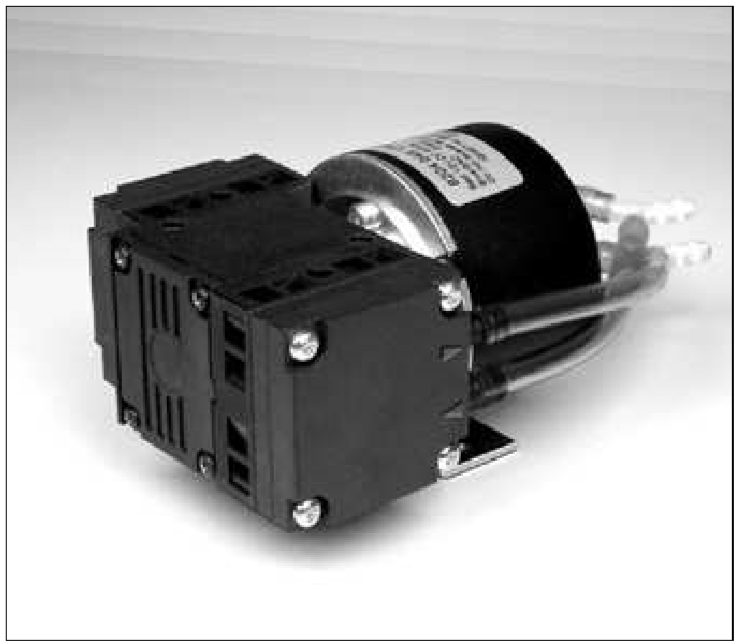
\includegraphics[width=6cm]{4-experiment-design/img/pump-850-1-2-kndc-b.png}
    \end{align*}
    \caption{KNF 850.1.2. KNDC B Miniature Diaphragm Pump.}\label{fig:pumppic}
\end{figure}


\begin{figure}[H]
    \begin{align*}
        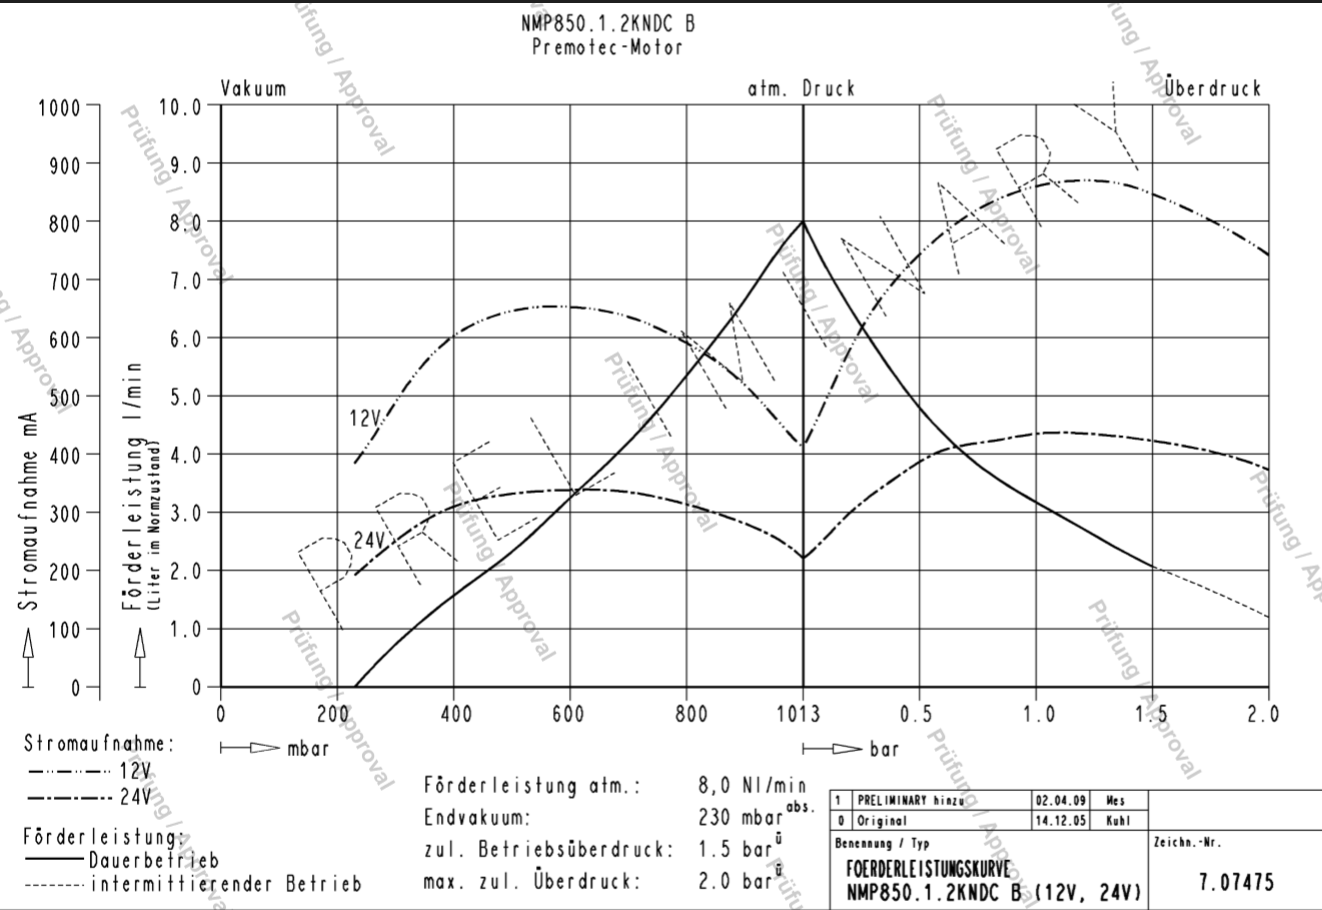
\includegraphics[width=15cm]{4-experiment-design/img/pump-flow-rate-current-graph.png}
    \end{align*}
    \caption{KNF 850.1.2. KNDC B Flow Rate and Current Draw to Pressure Graph.}\label{fig:pumpflowcur}
\end{figure}


\subsubsection{Electromagnetically Controlled Valves}
Filling the sampling bags will be controlled by solenoid valves. The solenoid valves which have been selected are model VDW23-5G-1-H-Q, seen in Figure \ref{fig:valve}, manufactured by SMC. These valves will be normally closed through out the experiment with zero power consumption and will open, when given power, to fill up the sampling bags at specific altitudes. In addition one valve will be on the CAC, in order to seal the coil at the end of the flight and another at the end of the AAC tubing, flushing valve, in order to flush the system.  The valves selected for these are model VDW22UANXB, Figure \ref{fig:valve}. The CAC valve will be opened shortly after take off and remain open the whole flight. This valve will be closed shortly before landing. The flushing valve will be opened before sampling in order to ensure the air in the tubes is from the correct altitude.

\begin{figure}[H]
    \begin{align*}
        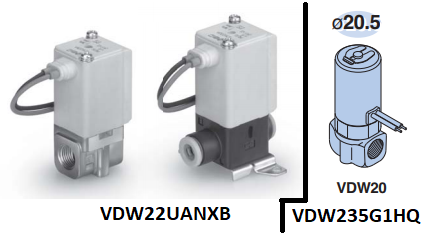
\includegraphics[width=6cm]{4-experiment-design/img/valves.png}
    \end{align*}
    \caption{SMC Solenoid Valves, VDW22UANXB on the Left, VDW23-5G-1-H-Q on the Right.}
    \label{fig:valve}
\end{figure}

The port size of the valves is 1/8" which is compatible with the gas analyzer. The coil inside can withstand temperatures from -20 to 50 °C which is suitable for flight operations at high altitudes. These valves can operate under a maximum pressure drop of 133 Pa. Valves from the same series have been flown before to the stratosphere and provided successful results \cite{LISA} however, the valves will be tested at low temperature and pressure to check they still operate as intended. These planned tests can be seen in Test 4, Table \ref{tab:vacuum-test} and Test 5, Table \ref{tab:thermal-test}.
 
\subsubsection{Switching Circuits}
The valves, pump and heaters will not be powered by the Arduino but they still need to be controlled by it. In order to allow this control a connection will be made for each component to the Arduino with a switching circuit. This switching circuit will use a eleven MOSFETs, model IRLB8748PBF, Figure \ref{fig:mosfet}, to control which components are turned on at which time.

\begin{figure}[H]
    \begin{align*}
        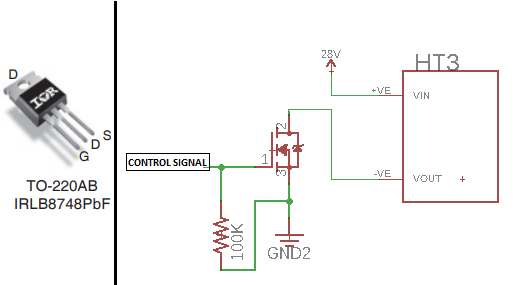
\includegraphics[width=10cm]{4-experiment-design/img/mosfet.png}
    \end{align*}
    \caption{Figure Showing an Image of the 30V,78A,75W MOSFET, Model Number IRLB8748PBF on the Left and the Schematic for the Switching Circuit for One Heater on the Right.}\label{fig:mosfet}
\end{figure}

\subsubsection{Schematic}

The schematics show all the components and how they are connected, the full schematics can be seen in Figure \ref{fig:Schematic}. There are four requirements for the the power distribution given below:

\begin{itemize}

    \item $28.8 \, V$ for the heaters.  
    
    \item $28.8 \, V \Longrightarrow 24 \, V$ for the pump and valves.
    
    \item $24 \, V \Longrightarrow 12 \, V$ for the airflow sensor and Arduino due.
    
    \item $3.3 \, V$ for the temperature, pressure and humidity sensors. 
    
\end{itemize}

The voltage available from gondola power is 28.8 V, therefore the heaters have been connected directly to the main power supply. For the rest of the components, two 24 V DC-DCs in parallel has been used to make sure if one of them fails then the other can take over. The circuitry can be seen in Figure \ref{fig:dc-dc-redun}. All the valves and the pump are then powered through the 24 V DC-DCs. To step down the voltage from 24 V to 12 V to power the airflow sensor and the Arduino, a voltage regulator has been used at the output of the DC-DCs. Finally, to power the temperature, humidity and pressure sensors, 3.3 V is required which is supplied by the Arduino board. 


\begin{figure}[H]
    \begin{align*}
        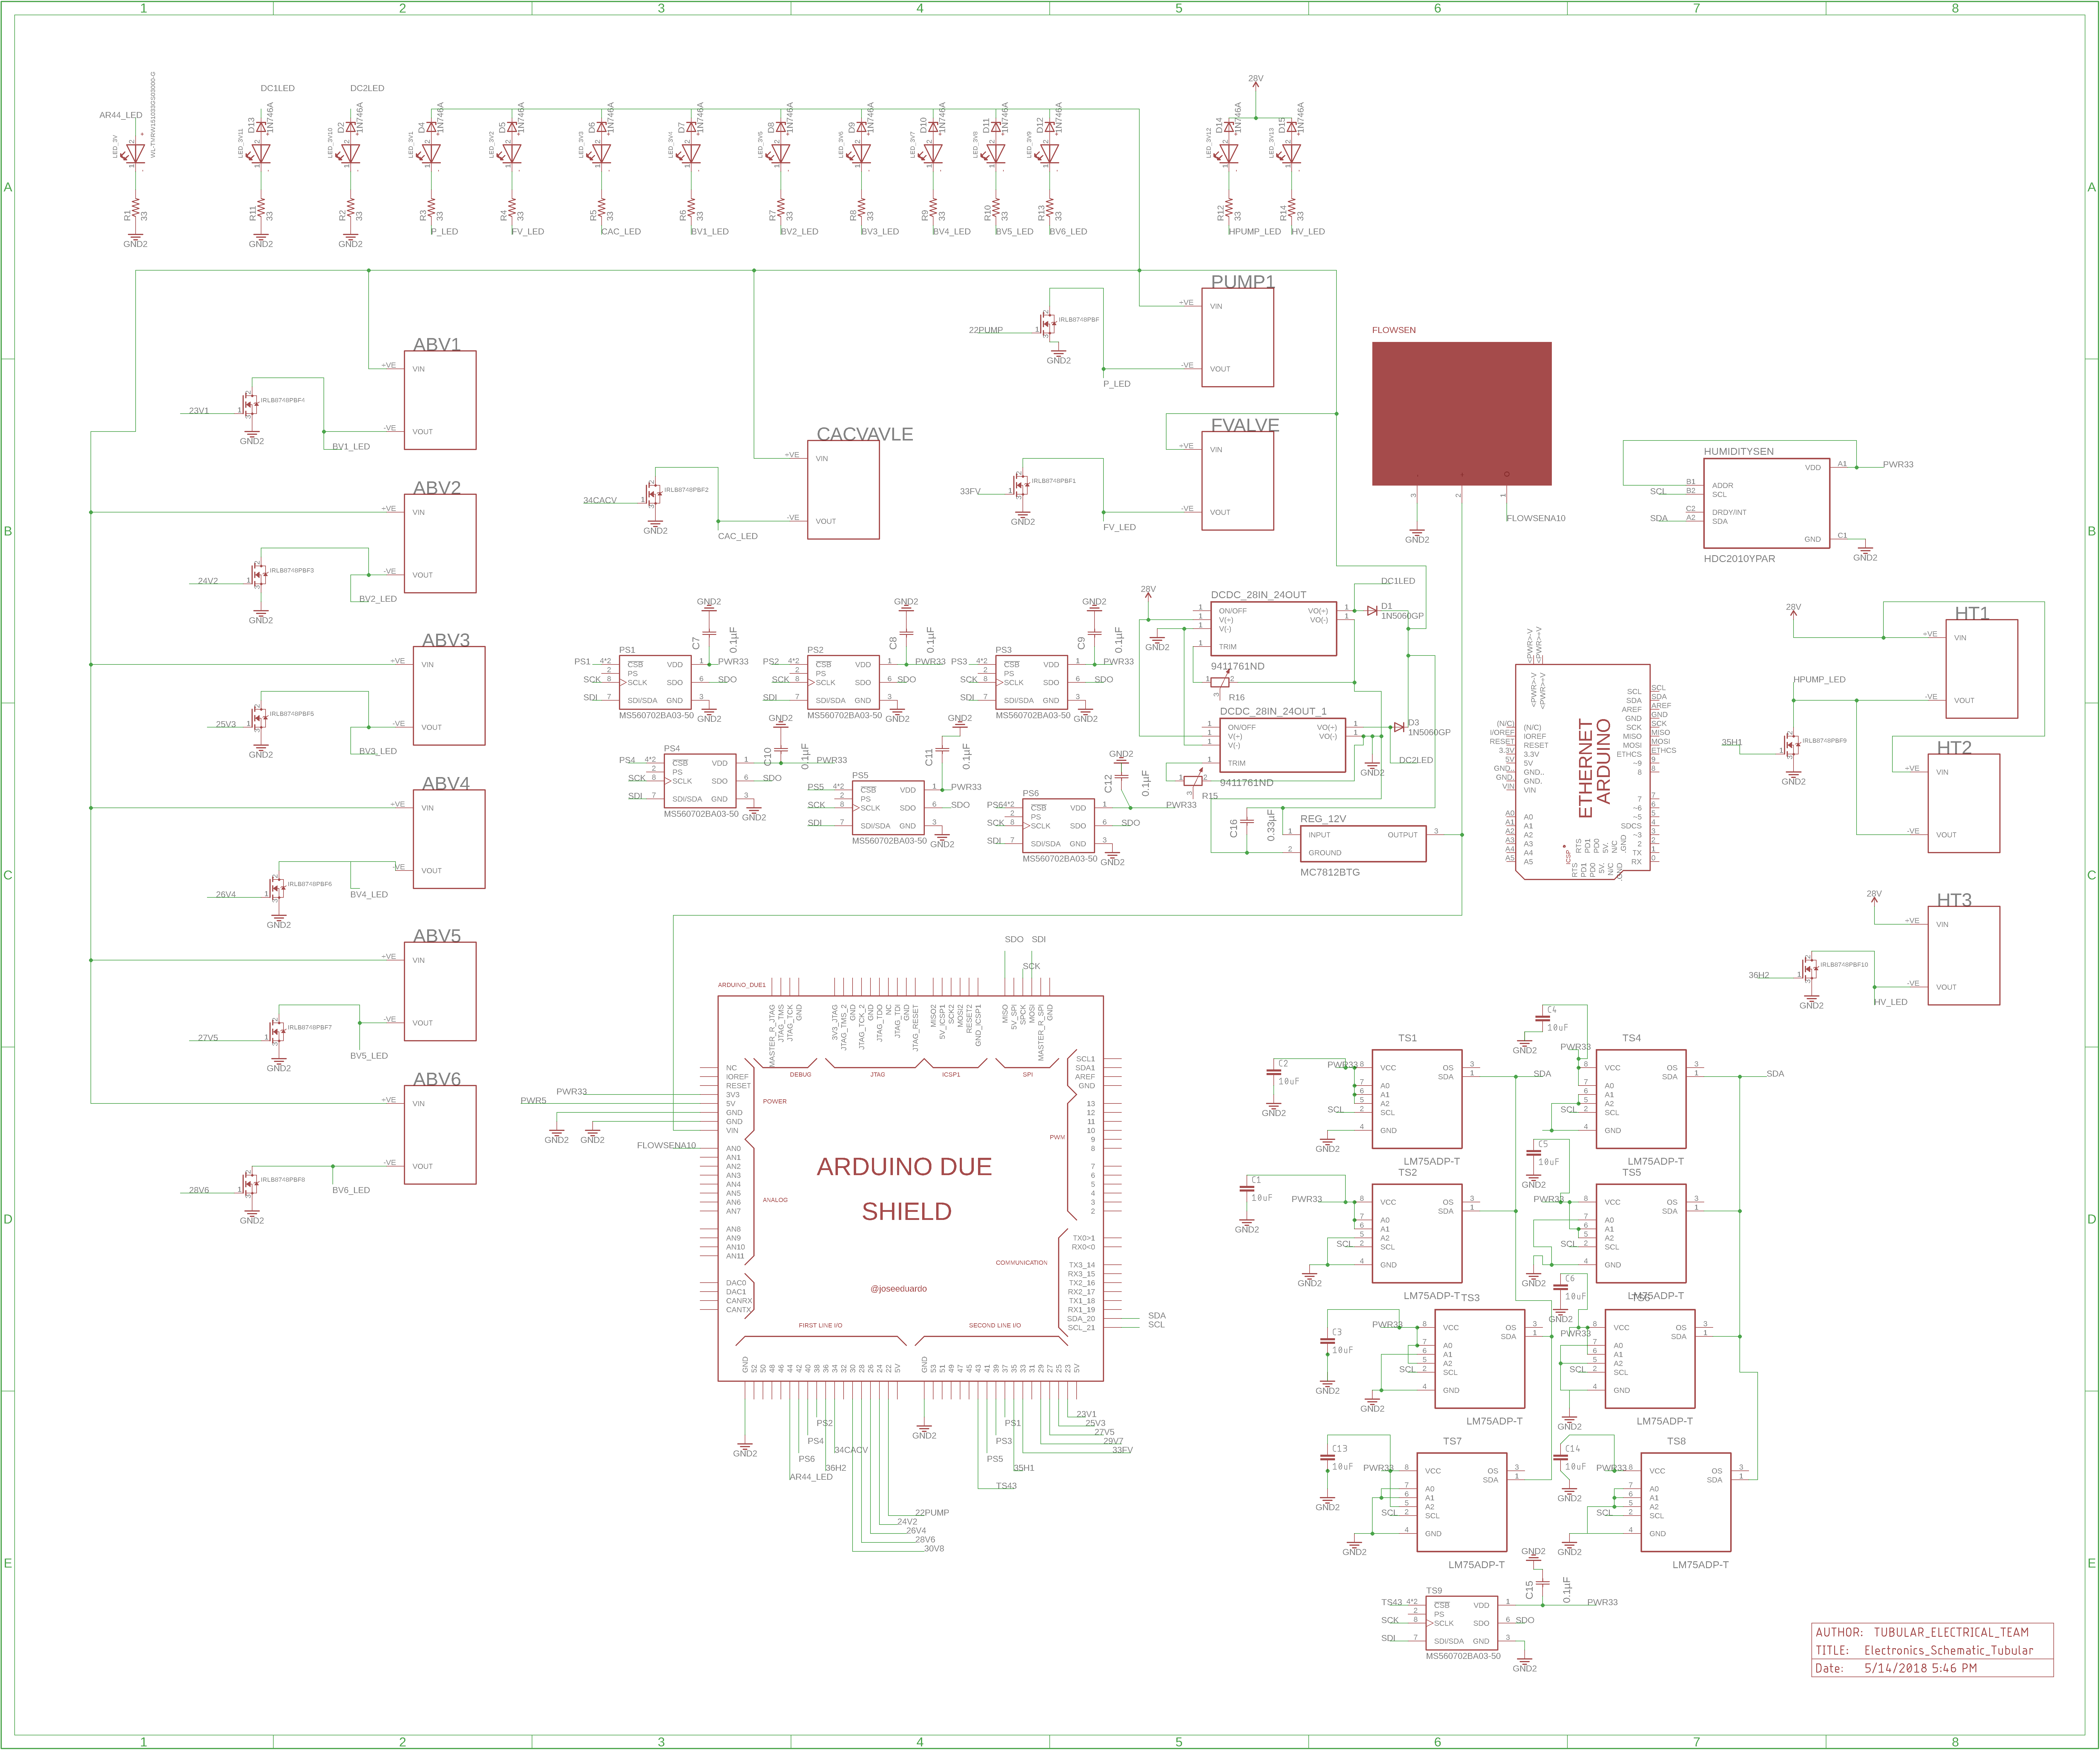
\includegraphics[width=16cm]{4-experiment-design/img/Schematics.png}
    \end{align*}
    \caption{Schematic for All of the Electronics on Board TUBULAR.}\label{fig:Schematic}
\end{figure}

\begin{figure}[H]
    \begin{align*}
        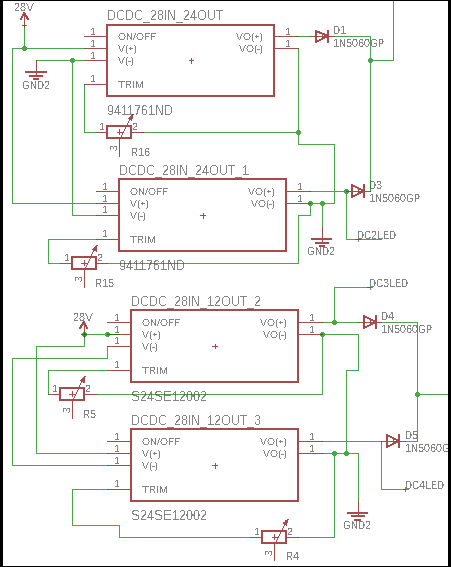
\includegraphics[width=16cm]{4-experiment-design/img/DCDC-converter-redundancy.png}
    \end{align*}
    \caption{Schematic Showing the DC-DC Redundancy of Both 24 V DC-DC Converters and the 12 V Voltage Regulator.}\label{fig:dc-dc-redun}
\end{figure}


\subsubsection{PCB Layout}

All electronic control circuits will be gathered on a single PCB on level 3 of the Brain. The PCB contains the Arduino due, switching circuits, indication LEDs, a temperature sensor, the power system and all necessary connectors. The connectors have been divided so that each connector's wires goes to the same level of the Brain to improve cable management. To further improve cable management the shared pins for I2C and SPI are connected to a single pin on each respective D-SUB connector and should be split up on the respective level. The PCB Layout can be seen in Figure \ref{fig:PCBLayout}.


\begin{figure}[H]
    \begin{align*}
        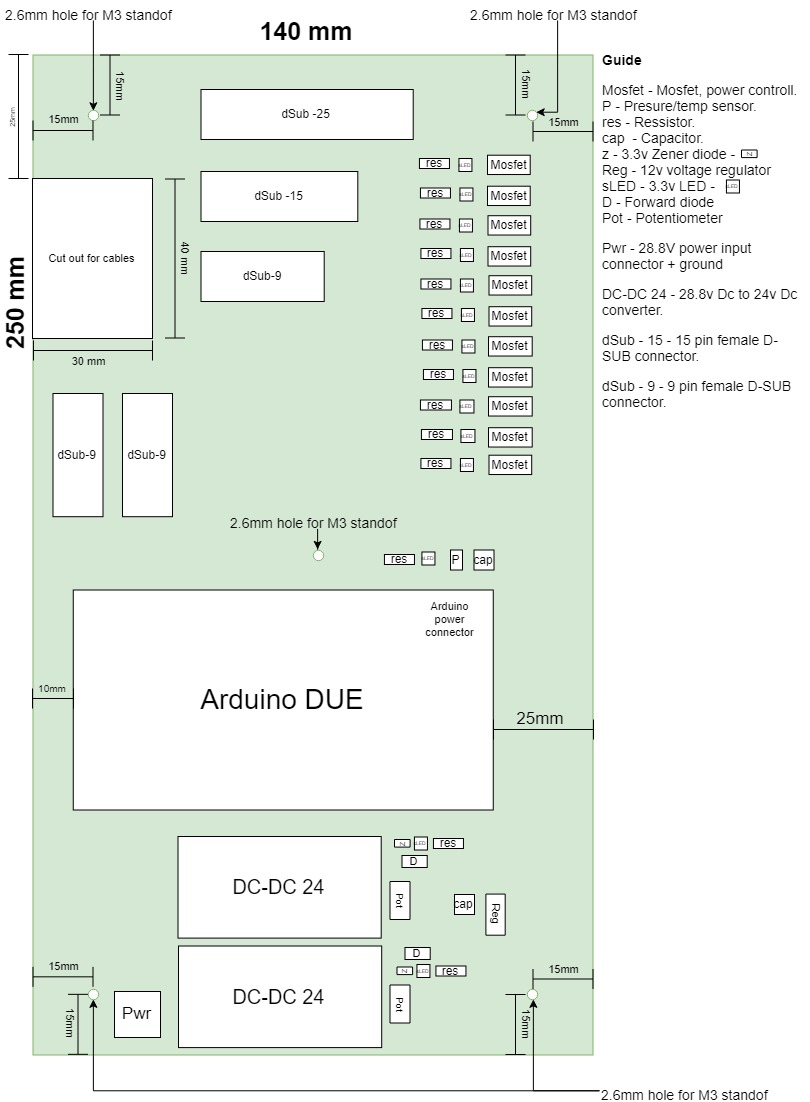
\includegraphics[width=0.9\textwidth]{4-experiment-design/img/PCB_Prelim_2.jpg}
    \end{align*}
    \caption{PCB Layout.}\label{fig:PCBLayout}
\end{figure}

The PCB was made using Eagle software. The traces has a width designed to fit the IPC-2221 standards\cite{IPC-2221B}. The PCB layout can be seen in in Section \ref{sec:pcbSchematics}. 




\raggedbottom